\section{«فرق بین Virtual address و raw-address»}
\label{sec:diff-virtual-raw}

\section{Virtual Address (آدرس مجازی)}
آدرس مجازی آدرسی است که برنامه یا نرم‌افزار آن را می‌بیند و استفاده می‌کند، اما خودش مستقلاً به حافظه دسترسی ندارد. در واقع، سیستم‌عامل و واحد مدیریت حافظه ($\text{MMU}$ -- Memory Management Unit) این آدرس‌ها را به آدرس واقعی در حافظه فیزیکی ($\text{Physical Address}$ یا $\text{Raw Address}$) ترجمه می‌کنند. این مکانیزم مزیت‌های متعددی دارد: هر برنامه تصور می‌کند که یک فضای حافظه مستقل در اختیار دارد، در حالی که همه برنامه‌ها از یک حافظه فیزیکی مشترک استفاده می‌کنند. علاوه بر این، وقتی برنامه‌ای از یک $\text{Virtual Address}$ استفاده می‌کند، $\text{MMU}$ آن را به آدرس واقعی تبدیل می‌کند تا داده مربوطه خوانده یا نوشته شود. چنین سیستمی امکان اجرای همزمان چند برنامه بدون تداخل و با حفظ امنیت حافظه را فراهم می‌کند.

\subsection{مثال کد Virtual Address}

\begin{lstlisting}[language=C, caption={مثالی از Virtual Address در برنامه C}, basicstyle=\ttfamily, keywordstyle=\color{blue}, commentstyle=\color{gray}, frame=single, breaklines=true]
#include <stdio.h>

int main() {
    int x = 42;
    printf("Address of x: %p\n", &x);
    return 0;
}
\end{lstlisting}

خروجی ممکن است چیزی شبیه این باشد:

\begin{verbatim}
Address of x: 0x7ffee4b2a98c
\end{verbatim}

این آدرس چاپ شده، یک $\text{Virtual Address}$ است که برنامه می‌بیند. سیستم‌عامل و $\text{MMU}$ آن را به یک آدرس واقعی در $\text{RAM}$ نگاشت می‌کنند.

\section{Raw Address (آدرس خام یا واقعی)}
آدرس خام یا واقعی، آدرسی است که به‌صورت مستقیم در حافظه فیزیکی یا در فایل باینری وجود دارد. برخلاف آدرس مجازی، هیچ ترجمه یا نگاشت مجازی برای آن انجام نمی‌شود. این نوع آدرس معمولاً در سطح سخت‌افزار یا هنگام تحلیل و دیباگ فایل‌های اجرایی (مانند استفاده از $\text{hex editor}$ یا $\text{linker}$) کاربرد دارد. آدرس‌های خام ثابت هستند و موقعیت داده‌ها در فایل یا حافظه فیزیکی تغییر نمی‌کند.

\subsection{مثال Raw Address}
فرض کنید یک فایل اجرایی ساده داریم که شامل متغیر داده‌ای زیر است:
\begin{lstlisting}[language=C, basicstyle=\ttfamily, frame=single]
int y = 100;
\end{lstlisting}

اگر این فایل را با $\text{Hex Editor}$ باز کنیم، داده ممکن است در $\text{offset}$ مشخصی از فایل ذخیره شده باشد، مثلاً:

\begin{verbatim}
Raw Address: 0x0030 (offset در فایل)
Data: 100 (int)
\end{verbatim}

این آدرس همان $\text{Raw Address}$ است که ثابت بوده و بدون ترجمه است. وقتی برنامه اجرا می‌شود، سیستم‌عامل و $\text{MMU}$ این $\text{Raw Address}$ را به یک $\text{Virtual Address}$ در حافظه نگاشت می‌کنند، مثلاً $\text{0x00402000}$.

\section{تعریف RVA}
$\text{RVA}$ یا \textbf{Relative Virtual Address} آدرس نسبی یک بخش از فایل نسبت به \textbf{Base Address} ماژول در حافظه است.

فرمول کلی:
\[
\text{Virtual Address} = \text{Base Address} + \text{RVA}
\]

\begin{itemize}
    \item \textbf{Base Address}: آدرس شروع ماژول در حافظه
    \item \textbf{RVA}: فاصله نسبی از ابتدای ماژول تا بخش مورد نظر
\end{itemize}

\textbf{مثال ساده:}
\begin{itemize}
    \item Base Address: \text{0x400000}
    \item RVA: \text{0x1000}
    \item Virtual Address واقعی: \text{0x401000}
\end{itemize}

\section{بخش‌های مرتبط در فایل PE}
در فایل‌های $\text{PE}$ (مثل $\text{EXE}$ و $\text{DLL}$)، $\text{RVA}$ برای اشاره به بخش‌های مختلف استفاده می‌شود:

\begin{center}
\begin{tabular}{|l|l|}
\hline
HDK & هدر فایل PE شامل Signature، File Header و Optional Header \\
\hline
LDO & بخش‌های قابل بارگذاری (Data, Code) \\
\hline
HL & بخش‌های حافظه پویا یا هدرهای اضافی \\
\hline
\end{tabular}
\end{center}

\section{نمونه محاسبات کامل RVA}
فرض کنید فایل $\text{PE}$ با مشخصات زیر داریم:

\begin{center}
\begin{tabular}{|l|l|}
\hline
Base Address & 0x400000 \\
.text Section RVA & 0x1000 \\
.text Section Size & 0x600 \\
.text PointerToRawData & 0x200 \\
.data Section RVA & 0x2000 \\
.data Section Size & 0x200 \\
.data PointerToRawData & 0x800 \\
\hline
\end{tabular}
\end{center}

نمادها و $\text{RVA}$ آنها:

\begin{center}
\begin{tabular}{|l|l|}
\hline
Symbol & RVA \\
\hline
func1 & 0x1010 \\
func2 & 0x1080 \\
globalVar & 0x2010 \\
\hline
\end{tabular}
\end{center}

\subsection{محاسبه Virtual Address (VA)}
\[
VA = BaseAddress + RVA
\]

\begin{center}
\begin{tabular}{|l|l|}
\hline
Symbol & VA \\
\hline
func1 & 0x401010 \\
func2 & 0x401080 \\
globalVar & 0x402010 \\
\hline
\end{tabular}
\end{center}

\subsection{محاسبه File Offset (FO)}
\[
FO = RVA - SectionRVA + PointerToRawData
\]

\begin{center}
\begin{tabular}{|l|l|}
\hline
Symbol & FO \\
\hline
func1 & 0x210 \\
func2 & 0x280 \\
globalVar & 0x810 \\
\hline
\end{tabular}
\end{center}

\section{نمودار تصویری PE}
\begin{center}
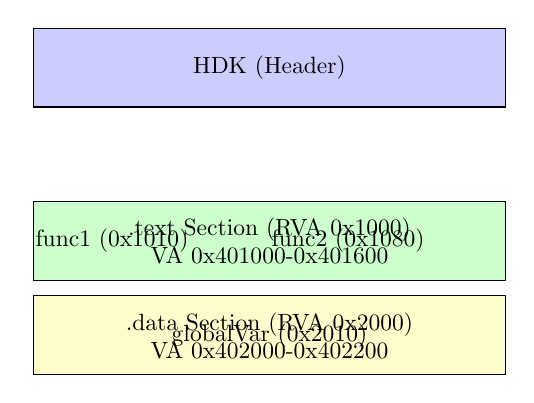
\begin{tikzpicture}[scale=1, every node/.style={scale=0.85}]
% Draw sections
\draw[fill=blue!20] (0,0) rectangle (6,1) node[pos=.5]{HDK (Header)};
\draw[fill=green!20] (0,-1.2) rectangle (6,-2.2) node[pos=.5, align=center]{.text Section (RVA 0x1000)\\VA 0x401000-0x401600};
\draw[fill=yellow!20] (0,-2.4) rectangle (6,-3.4) node[pos=.5, align=center]{.data Section (RVA 0x2000)\\VA 0x402000-0x402200};

% Symbols
\node at (1,-1.7) {func1 (0x1010)};
\node at (4,-1.7) {func2 (0x1080)};
\node at (3,-2.9) {globalVar (0x2010)};
\end{tikzpicture}
\end{center}

\section{اهمیت}
$\text{RVA}$ اساس کار دی‌کامپایلرها، دیباگرها و ابزارهای مهندسی معکوس است و کمک می‌کند بخش‌های مختلف فایل $\text{PE}$ را در حافظه یا روی دیسک به درستی پیدا کنیم.

\section{دیاگرام نگاشت فایل‌ها در حافظه و دیسک}

\subsection{File on Disk (فایل روی دیسک)}
داده‌ها روی دیسک به بلوک‌ها (Blocks / Sectors) تقسیم شده‌اند.
هر بلوک اندازه مشخصی دارد (مثلاً 4 کیلوبایت).

\subsection{RAM / Memory (حافظه اصلی)}
بلوک‌ها هنگام دسترسی به برنامه، در Buffer یا Page در حافظه بارگذاری می‌شوند.
اگر از Memory-mapped file استفاده شود، بلوک‌ها مستقیماً روی فضای آدرس برنامه نگاشت می‌شوند.

\subsection{File System Cache / Page Cache}
سیستم‌عامل اغلب داده‌ها را در کش حافظه ذخیره می‌کند تا دفعات بعد نیاز به خواندن از دیسک نباشد.
به این ترتیب خواندن و نوشتن سریع‌تر می‌شود.

\subsection{CPU Access}
برنامه به Buffer یا Memory-mapped Page دسترسی دارد و می‌تواند داده‌ها را بخواند یا تغییر دهد.
در حالت Memory-mapped, تغییر داده در حافظه می‌تواند مستقیماً روی دیسک هم منعکس شود.

\subsection{نکات مهم}
\begin{itemize}
    \item \textbf{تفاوت Buffered I/O و Memory-mapped:}
    Buffered I/O: داده‌ها بلوک‌بلوک از دیسک خوانده و نوشته می‌شوند، با کنترل بیشتر روی I/O.
    Memory-mapped: داده‌ها در فضای آدرس حافظه برنامه نگاشت می‌شوند، دسترسی مستقیم و سریع است.
    
    \item \textbf{Page / Block Mapping:}
    حافظه به صفحات (Page) و دیسک به بلوک‌ها (Block) تقسیم می‌شوند.
    نگاشت صفحه‌ها و بلوک‌ها توسط سیستم‌عامل مدیریت می‌شود.
\end{itemize}

\subsection{دیاگرام نگاشت فایل به حافظه}

\begin{center}
\begin{tikzpicture}[>=stealth', node distance=2.5cm, auto]

% Styles definition locally for this diagram
\tikzstyle{block} = [rectangle, draw, text width=6em, text centered, minimum height=2em]
\tikzstyle{line} = [draw, -latex']

% Nodes
\node [block] (disk) {File on Disk\\(Block 0,1,2,...)};
\node [block, right of=disk, node distance=5cm] (ram) {RAM (Memory)\\Buffer/Page 0,1,2,...};
\node [block, below of=disk, node distance=3cm] (cache) {File System Cache / Page Cache};
\node [block, right of=cache, node distance=5cm] (cpu) {CPU Access};

% Arrows
\path [line] (disk) -- (ram);
\path [line] (disk) -- (cache);
\path [line] (cache) -- (ram);
\path [line] (ram) -- (cpu);

% Labels
\node [above of=disk, node distance=1.5cm] {Disk Blocks};
\node [above of=ram, node distance=1.5cm] {Memory Pages / Buffers};

\end{tikzpicture}
\end{center}